\numberwithin{equation}{section}

\subsection{Histograms}
%\begin{frame}
  %\frametitle{Outline}
  %\tableofcontents[ currentsection ]
%\end{frame}

\begin{frame}{Description of Simulations}

  Describe what was done for the following two sets of histograms.

\end{frame}


\begin{frame}{Results}
 

  \begin{columns}[t]
    \column{.5\textwidth} 
    %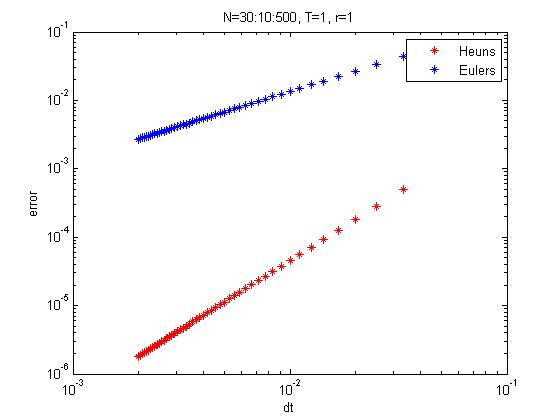
\includegraphics[width=6cm]{img/Heun500}
    histogram from Matlab simulations
    \column{.5\textwidth}
    %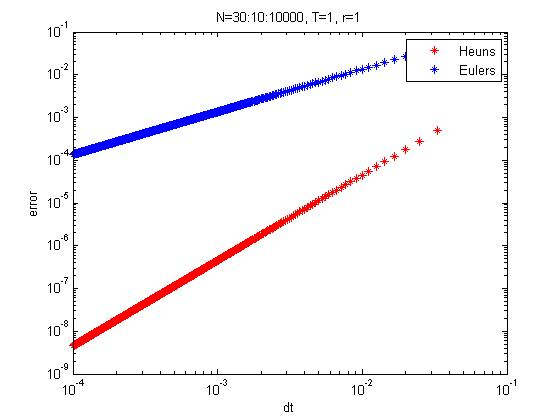
\includegraphics[width=6cm]{img/Heun10000}
    histogram from C simulations
  \end{columns}


\end{frame}



\subsection{Approximations}

\begin{frame}{Milstein Method}

    \textbf{This is not correct.}

	\begin{itemize}
		\item Technique for the approximate numerical solution of a stochastic differential equation
		\item Increases accuracy by using It\^o's Formula by adding the second-order term
	\end{itemize} 

	\begin{align*}
		Y_{i+1} = Y_i +b\delta t + \sigma \delta W_t + \frac{1}{2} \sigma \sigma_x \{(\delta W_t)^2 - \delta t\} 
	\end{align*}

\end{frame}

\begin{frame}{Full Approximations}
RESULTS \\
Because this is a random variable each time it's run it's different. \\
MOVIE INSERT 
\end{frame}

\begin{frame}{Confidence Intervals}

  \textbf{I have no idea what this means or what was done???}

  In order to better analyze our data we want to calculate our
  confidence intervals. 
  To do this we needed to come up with a formula to calculate them. \\

  $$\hat{\theta} - S(\hat{\theta}) L \leq \theta \leq \hat{\theta} + S(\hat{\theta}) L$$ \\
\end{frame}

\begin{frame}{Experimental Design}

  \textbf{What is $n_1$? Where is the ``following formula?''}

  We need to estimate the number of trials. To do this we solved the following formula for $n_1$
  and multiplied by the number of frequency tables we have.

\vfill

Our frequency tables are divided into three groups:
\begin{itemize}
	\item species 1 lives while species 2 dies out
	\item species 2 lives while species 1 dies out
	\item species 1 and species 2 lives
\end{itemize}

\vfill 

\end{frame}

\begin{frame}{Solving For The Number of Trials}

  \textbf{You ``found'' L? Was it hiding?}

  By letting $P_1 = \frac{1}{2}$ and finding $L = 5.991465$ in R, we get:

  $$\sqrt{\frac{P_1 (1-P_1)}{n_1}} \ L = .01$$ \\
  $$n_1 = \frac{L^2 P_1 (1-P_1)}{.0001}$$ \\
  After multiplying by $3$ (our number of frequency tables) we get: \\
  \begin{center} 
    $N = 44935.9875$ 
  \end{center} 

  From this we knew to run our program $45,000$ times. 
\end{frame}


